\documentclass[fsharpnotes.tex]{subfiles}
\graphicspath{ {./figures/} }

\begin{document}
\chapter{Testing Programs}
\label{chap:testing}
A software bug is an error in a computer program that causes it to produce an incorrect result or behave in an unintended manner. The term 'bug' was used by Thomas Edison in 1878\footnote{\url{https://en.wikipedia.org/wiki/Software_bug}}\footnote{\url{http://edison.rutgers.edu/NamesSearch/DocImage.php3?DocId=LB003487}}, but made popular in computer science by Grace Hopper, who found a moth interfering with the electronic circuits of the Harward Mark II electromechanical computer and coined the term \idx{bug} for errors in computer programs. The original bug is shown in \Cref{fig:bug}.
\begin{figure}
  \centering
  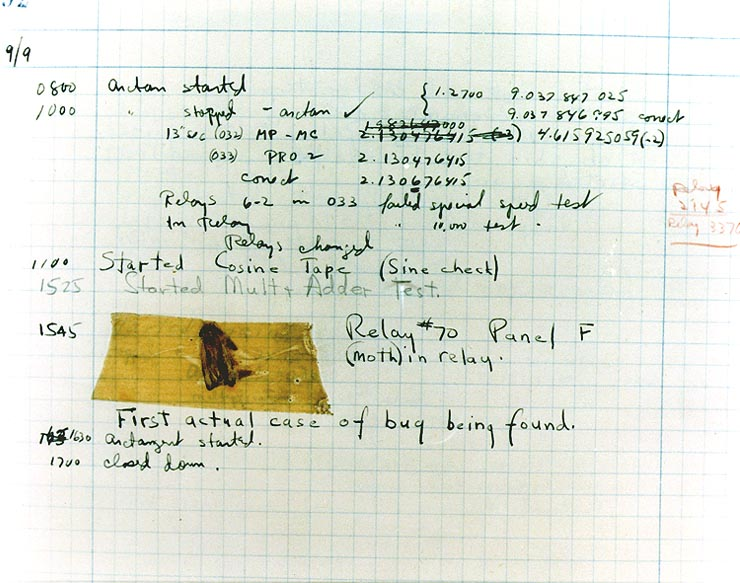
\includegraphics[width=0.45\linewidth]{H96566k}
  \caption{The first computer bug, caught by Grace Hopper, U.S. Naval Historical Center Online Library Photograph NH 96566-KN.}
  \label{fig:bug}
\end{figure}
Software is everywhere, and errors therein have a huge economic impact on our society and can threaten lives\footnote{\url{https://en.wikipedia.org/wiki/List_of_software_bugs}}.

The ISO/IEC organizations have developed standards for software testing\footnote{ISO/IEC 9126, International standard for the evaluation of software quality, December 19, 1991, later replaced by ISO/IEC 25010:2011}.  To illustrate basic concepts of software quality, consider a hypothetical route planning system. Essential factors of its quality are:
\begin{description}
\item[Functionality:]\idxs{functionality} Does the software compile and run without internal errors. Does it solve the problem it was intended to solve? E.g., does the route planning software find a suitable route from point a to b?
\item[Reliability:]\idxs{reliability} Does the software work reliably over time? E.g., does the route planning software work when there are internet dropouts?
\item[Usability:]\idxs{usability} Is the software easy and intuitive to use by humans? E.g., is it easy to enter addresses and alternative routes in the software's interface?
\item[Efficiency:]\idxs{efficiency} How many computer and human resources does the software require? E.g., does it take milliseconds or hours to find a requested route? Can the software run on a mobile platform with limited computer speed and memory?
\item[Maintainability:]\idxs{maintainability} In case of the discovery of new bugs, is it easy to test and correct the software? Is it easy to extend the software with new functionality? E.g., is it easy to update the map with updated roadmaps and new information? Can the system be improved to work both for car drivers and bicyclists? 
\item[Portability:]\idxs{portability} Is it easy to port the software to new systems such as new server architecture and screen sizes? E.g., if the routing software originally was written for IOS devices, will it be easy to port to Android systems?
\end{description}
The above-mentioned concepts are ordered based on the requirements of the system. Functionality and reliability are perhaps the most important concepts, since if the software does not solve the specified problem, then the software design process has failed. However, many times the problem definition will evolve along with the software development process. But as a bare minimum, the software should run without internal errors and not crash under a well-defined set of circumstances. Furthermore, it is often the case that software designed for the general public requires a lot of attention to the usability of the software, since in many cases non-experts are expected to be able to use the software with little or no prior training. On the other hand, software used internally in companies will be used by a small number of people who become experts in using the software, and it is often less important that the software is easy to understand by non-experts. An example is text processing software like Microsoft Word versus Gnu Emacs and LaTeX. Word is designed to be used by non-experts for small documents such as letters and notes and relies heavily on interfacing with the system using click-interaction. On the other hand, Emacs and LaTeX are for experts for longer and professionally typeset documents and relies heavily on keyboard shortcuts and text-codes for typesetting document entities. 

The purpose of \idx{software testing} is to find bugs. When errors are found, then we engage in \idx{debugging}, which is the process of diagnosing and correcting bugs. Once we have a failed software test, i.e., one that does not find any bugs, then we have strengthened our belief in the software, but it is important to note that software testing and debugging rarely removes all bugs, and with each correction or change of software there is a fair risk new bugs being introduced. It is not exceptional that the testing-software is as large as the software being tested.

In this chapter, we will focus on two approaches to software testing which emphasize functionality: \idx[white-box testing]{white-box} and \idx{black-box testing}. An important concept in this context is \idx{unit testing}, where the program is considered in smaller pieces, called units, and for which accompanying programs for testing can be made which test these units automatically. Black-box testing considers the problem formulation and the program interface, and can typically be written early in the software design phase. In contrast, white-box testing considers the program text, and thus requires the program to be available. Thus, there is a tendency for black-box test programs to be more stable, while white-box testing typically is developed incrementally alongside the software development.

To illustrate software testing, we'll start with a problem:
\begin{problem}
  Given any date in the Gregorian calendar, calculate the day of the week.
\end{problem}
Facts about dates in the Gregorian calendar are:
\begin{itemize}
\item Combinations of dates and weekdays repeat themselves every 400 years.
\item The typical length of the months January, February, \dots follow the knuckle rule, i.e., January belongs to the index knuckle, February to the space between the index and the middle finger, and August restarts or starts on the other hand. All knuckle months have 31 days, all spacing months have 30 days except February, which has 29 days on leap years and 28 days all other years.
\item A leap year is a multiple of 4, except if it is also a multiple of 100 but not of 400.
\end{itemize}
Many solutions to the problem have been discovered, and here we will base our program on Gauss' method, which is based on integer division and calculates the weekday of the 1st of January of a given year. For any other date, we will count our way through the weeks from the previous 1st of January. The algorithm relies on an enumeration of weekdays starting with Sunday = 0, Monday = 1, \dots, and Saturday = 6. Our proposed solution is shown in \Cref{date2Day}.\jon{This example relies on lists, which has not been introduced yet.}
% 
\fsharp{date2Day.fsx}{date2Day}{A function that can calculate day-of-week from any date in the Gregorian calendar.}
% 
% To solve this problem, we are going to implement the Doomsday algorithm by John Conway\footnote{\url{http://www.timeanddate.com/date/doomsday-weekday.html}}. The algorithm is based on the fact that calendars repeat themselves every 400 years, and within a cycle, certain dates are always the same day of week. For the 400-year cycle, 1800-2199, the algorithm uses anchor days: 1800 - 1899: Friday, 1900 - 1999: Wednesday, 2000 - 2099: Tuesday, and 2100 - 2199: Sunday. For a given date (dd, mm, yyyy), the algorithm calculates the Doomsday of the year in question as by 6 steps:
% \begin{enumerate}
% \item Let $a$ be the integer division of the last two digits of yyyy by 12
% \item Let $b$ be the remainder of the last two digits of yyyy by 12
% \item Let $c$ be the integer division of $b$ by 4
% \item Let $d$ be the anchor number of yyyy
% \item Let $e$ be the remainder of $a+b+c+d$ by 7. This is the doomsday.
% \item count weekdays from nearest doomsday.
% \end{enumerate}

\section{White-box Testing}
\idx[white-box testing]{White-box testing} considers the text of a program. The degree to which the text of the program is covered in the test is called the \idx{coverage}. Since our program is small, we have the opportunity to ensure that all functions are called at least once, which is called \idx{function coverage}, and we will also be able to test every branching in the program, which is called \idx{branching coverage}. If both are fulfilled, we say that we have \idx{statement coverage}. The procedure is as follows:
\begin{enumerate}
\item Decide which units to test: The program shown in \Cref{date2Day} has 3 functions, and we will consider these each as a unit, but we might as well just have chosen \lstinline!date2Day! as a single unit. The important part is that the union of units must cover the whole program text, and since \lstinline!date2Day! calls both \lstinline!januaryFirstDay! and \lstinline!sum!, designing test cases for the latter two is superfluous. However, we may have to do this anyway when debugging, and we may choose at a later point to use these functions separately, and in both cases, we will be able to reuse the testing of the smaller units.
\item Identify branching points: The function \lstinline!januaryFirstDay! has no branching function, \lstinline!sum! has one, and depending on the input values, two paths through the code may be used, and \lstinline!date2Day! has one where the number of days in February is decided. Note that in order to test this, our test-date must be March 1 or later. In this example, there are only examples of \keyword{if}-branch points, but they may as well be loops and pattern matching expressions. In the \Cref{date2DayAnnotated} it is shown that the branch points have been given a comment and a number.
  % 
  \fsharp{date2DayAnnotated.fsx}{date2DayAnnotated}{In white-box testing, the branch points are identified.}
  % 
 \item For each unit, produce an input set that tests each branch: In our example, the branch points depend on a Boolean expression, and for good measure, we are going to test each term that can lead to branching. Using 't' and 'f' for \lstinline{true} and \lstinline{false}, we thus write,
   \begin{center}
     \rowcolors{2}{oddRowColor}{evenRowColor}
     \begin{tabularx}{\linewidth}{|l|l|p{3.5cm}|l|X|}
     \hline
     \rowcolor{headerRowColor} Unit & Branch & Condition & Input & Expected output\\
     \hline
       \lstinline{januaryFirstDay} & 0 & -& \lstinline{2016} & \lstinline{5}\\
     \hline
     \lstinline{sum} 
       & 1 & \lstinline{0 <= j} \lstinline{\&\&}\newline\hspace*{0.5em}\lstinline{j < lst.Length} &&\\
       & 1a & \lstinline{t \&\& t} & \lstinline{[1; 2; 3] 1} & \lstinline{3}\\
       & 1b & \lstinline{f \&\& t} & \lstinline{[1; 2; 3] -1} & \lstinline{0}\\
       & 1c & \lstinline{t \&\& f} & \lstinline{[1; 2; 3] 10} & \lstinline{0}\\
       & 1d & \lstinline{f \&\& f} & - & -\\
       \hline
       \lstinline{date2Day} & 1 & \lstinline{(y \% 4 = 0)} \lstinline{\&\&}\newline
       \hspace*{0.5em}\lstinline{((y \% 100 <> 0)}\newline
       \hspace*{1em}\lstinline{||}\newline
       \hspace*{1.5em}\lstinline{(y \% 400 = 0))} &  & \\
        & - & \lstinline{t \&\& (t || t)} & - & -\\
        & 1a & \lstinline{t \&\& (t || f)} & \lstinline{8 9 2016} & \lstinline{Thursday}\\
        & 1b & \lstinline{t \&\& (f || t)} & \lstinline{8 9 2000} & \lstinline{Friday}\\
        & 1c & \lstinline{t \&\& (f || f)} & \lstinline{8 9 2100} & \lstinline{Wednesday}\\
        & - & \lstinline{f \&\& (t || t)} & - & -\\
        & 1d & \lstinline{f \&\& (t || f)} & \lstinline{8 9 2015} & \lstinline{Tuesday}\\
        & - & \lstinline{f \&\& (f || t)} & - & -\\
        & - & \lstinline{f \&\& (f || f)} & - & -\\
       \hline
     \end{tabularx}
   \end{center}
   The impossible cases have been intentionally blank, e.g., it is not possible for $j<0$ and $j>n$ for some positive value $n$.
 \item Write a program that tests all these cases and checks the output, see ~\Cref{date2DayWhiteTest}.
   % 
   \fs[firstline=22]{date2DayWhiteTest}{The tests identified by white-box analysis. The program from \Cref{date2DayAnnotated} has been omitted for brevity.}
   % 
\end{enumerate}
Notice that the output of the tests is organized such that they are enumerated per unit, hence we can rearrange as we like and still uniquely refer to a unit's test. Also, the output of the test program produces a list of tests that should return true or success or a similar positively loaded word, but without further or only little detail, such that we at a glance can identify any test that produced unexpected results.

After the white-box testing has failed to find errors in the program, we have some confidence in the program, since we have run every line at least once. It is, however, in no way a guarantee that the program is error free, which is why white-box testing is often accompanied with black-box testing to be described next.

\section{Black-box Testing}
In black-box testing, the program is considered a black box, and no knowledge is required about how a particular problem is solved. In fact, it is often useful not to have that knowledge at all. It is rarely possible to test all input to a program, so in black-box testing, the solution is tested for typical and extreme cases based on knowledge of the problem. The procedure is as follows:
\begin{enumerate}
\item Decide on the interface to use: It is useful to have an agreement with the software developers about what interface is to be used, e.g., in our case, the software developer has made a function \lstinline!date2Day d m y! where \lstinline!d!, \lstinline!m!, and \lstinline!y! are integers specifying the day, month, and year.
\item Make an overall description of the tests to be performed and their purpose:
  \begin{enumerate}[label=\arabic*]
  \item\label{allWeekDays} a consecutive week, to ensure that all weekdays are properly returned
  \item\label{crossBondaries} two set of consecutive days across boundaries that may cause problems: across a new year, and across a regular month boundary.
  \item\label{februaryBoundaries} a set of consecutive days across February-March boundaries for a leap and non-leap year
  \item\label{leapYears} four dates after February in a non-leap year, a non-multiple-of-100 leap year, a multiple-of-100-but-not-of-400 non-leap year, and a multiple-of-400 leap year.
  \end{enumerate}
  Given no information about the program's text, there are other dates that one could consider as likely candidates for errors, but the above is judged to be a fair coverage.
\item Choose a specific set of input and expected output relations on the tabular form:
\begin{center}
  \rowcolors{2}{oddRowColor}{evenRowColor}
  \begin{tabular}{|l|r|l|}
    \hline
    \rowcolor{headerRowColor} Test number&Input& Expected output\\
    \hline
    \ref{allWeekDays}a&1 1 2016&Friday\\
    \ref{allWeekDays}b&2 1 2016&Saturday\\
    \ref{allWeekDays}c&3 1 2016&Sunday\\
    \ref{allWeekDays}d&4 1 2016&Monday\\
    \ref{allWeekDays}e&5 1 2016&Tuesday\\
    \ref{allWeekDays}f&6 1 2016&Wednesday\\
    \ref{allWeekDays}g&7 1 2016&Thursday\\
    \hline
    \ref{crossBondaries}a&31 12 2014&Wednesday\\
    \ref{crossBondaries}b&1 1 2015&Thursday\\
    \ref{crossBondaries}c&30 9 2017&Saturday\\
    \ref{crossBondaries}d&1 10 2017&Sunday\\
    \hline
    \ref{februaryBoundaries}a&28 2 2016&Sunday\\
    \ref{februaryBoundaries}b&29 2 2016&Monday\\
    \ref{februaryBoundaries}c&1 3 2016&Tuesday\\
    \ref{februaryBoundaries}d&28 2 2017&Tuesday\\
    \ref{februaryBoundaries}e&1 3 2017&Wednesday\\
    \hline
    \ref{leapYears}a&1 3 2015&Sunday\\
    \ref{leapYears}b&1 3 2012&Thursday\\
    \ref{leapYears}c&1 3 2000&Wednesday\\
    \ref{leapYears}d&1 3 2100&Monday\\
    \hline
  \end{tabular}
\end{center}
\item Write a program executing the tests, as shown in \Cref{date2DayBlackTestCode,date2DayBlackTest}.
% 
\fsharp[firstline=28,firstnumber=28]{date2DayBlackTest.fsx}{date2DayBlackTestCode}{The tests identified by black-box analysis. The program from \Cref{date2DayAnnotated} has been omitted for brevity.}
%
\fsOutput{date2DayBlackTest}{Output from \Cref{date2DayBlackTestCode}.} 
%
Notice how the program has been made such that it is almost a direct copy of the table produced in the previous step.
\end{enumerate}
A black-box test is a statement of what a solution should fulfill for a given problem. Hence, \advice{it is a good idea to make a black-box test early in the software design phase, in order to clarify the requirements for the code to be developed and take an outside view of the code prior to developing it.}

After the black-box testing has failed to find errors in the program, we have some confidence in the program, since, from a user's perspective, the program produces sensible output in many cases. It is, however, in no way a guarantee that the program is error free.

\begin{comment}
  http://www.scientificamerican.com/article/pogue-5-most-embarrassing-software-bugs-in-history/, 5 Most Embarrassing Software Bugs in History

  http://royal.pingdom.com/2009/03/19/10-historical-software-bugs-with-extreme-consequences/

  https://raygun.com/blog/2014/05/10-costly-software-errors-history/

  http://www.computerworld.com/article/2515483/enterprise-applications/epic-failures--11-infamous-software-bugs.html

  http://catless.ncl.ac.uk/Risks/20.59.html#subj1

  https://en.wikipedia.org/wiki/List_of_software_bugs

  December 19, 1991; ISO/IEC 9126, the international standard for the evaluation of software quality, replaced by ISO/IEC 25010:2011. Not publicly available, \footnote{A review of the ISO/IEC 9126 is given in \url{http://www.sqa.net/iso9126.html}. A brief review of ISO/IEC 25010:2011 is given in }
\end{comment}

\section{Debugging by Tracing}
\label{sec:tracing}
Once an error has been found by testing, the \idx{debugging} phase starts. The cause of a bug can either be that the chosen algorithm is the wrong one for the job, or the implementation of it has an error. In the debugging process, we have to keep an open mind and not rely on assumptions, since assumptions tend to blind the reader of a text. A frequent source of errors is that the state of a program is different than expected, e.g., because the calculation performed is different than intended, or that the return of a library function is different than expected. The most important tool for debugging is \emph{simplification}. This is similar to white-box testing, but where the units tested are very small. E.g., the suspected piece of code could be broken down into smaller functions or code snippets, which are given well-defined input, and, e.g., use \lstinline!printfn! statements to obtain the output of the code snippet. Another related technique is to use \idx{mockup code}, which replaces parts of the code with code that produces safe and relevant results. If the bug is not obvious, then more rigorous techniques must be used, such as \idx{tracing}. Some development interfaces have a built-in tracing system, e.g., \lstinline[language=console]{fsharpi} will print inferred types and some binding values. However, often the source of a bug is due to a misunderstanding of the flow of data through a program execution, and we will in the following introduce \idx{Trace by hand} as a technique to simulate the execution of a program by hand. In the following, tracing will refer to the Trace by hand method.

To understand the method of Tracing by hand, we will consider 3 imperative programs of gradually increasing complexity: Firstly a program using function call, then one including a \lstinline{for}-loop, and finally one with dynamic scope. In \Cref{sec:recursiveTracing} is given a fourth example using recursion, a concept to be introduced in \Cref{sec:recursion}.

Tracing may seem tedious in the beginning, but in conjunction with strategically placed debugging \lstinline!printfn! statements, it is a very valuable tool for debugging.

\subsection{Tracing Function Calls}
Consider the program in \Cref{lexicalScopeTracing}.
%
\fs{lexicalScopeTracing}{Example of lexical scope and closure environment.}
%
The program calls \lstinline{testScope 2.0}, and by running the program, we see that the return-value is \lstinline{6.0} and not \lstinline{8.0}, as we had expected. Hence, we will use tracing to understand the result.

Tracing a program by hand means that we simulate its execution and, as part of that, keep track of the bindings, assignments closures, scopes, and input and output of the program. To do this, we need to consider the concept of \idx[environment]{environments}.

Environments describe bindings available to the program at the present scope and at a particular time and place in the code. There is always an outer environment, called $E_0$, and each time we call a function or create a scope, we create a new environment. Only one environment can be active at a time, and it is updated as we simulate the execution of code with new bindings and temporary evaluations of expressions. Once a scope is closed, then its environment is deleted and a return-value is transported to its enclosing environment. In tracing, we treat return-values explicitely. Likewise, output from, e.g., \lstinline{printfn} is reported with a special notation.

To trace code, we make a table with 4 columns: Step, Line, Environment, and Bindings and evaluations. The Step column we use to enumerate the steps performed. The Line column contains the program-line treated in a step {\em where} the present environment is updated. The Environment contains the name of the present environment, and Bindings $\ldots$ shows {\em what}  in the environment is updated.

The code in \Cref{lexicalScopeTracing} contains a function definition and a call, hence, the first lines of our table looks like,
\begin{center}
  \begin{tabular*}{0.9\linewidth}{l|lll}
    Step & Line & Env.\ & Bindings and evaluations\\
    \hline
    0 & - & $E_0$ & ()\\
    1 &\ref{lexicalScopeTracing:testScope} & $E_0$ & $\text{testScope} = \big((x), \text{testScope-body}, ()\big)$\\
    2 &\ref{lexicalScopeTracing:print} & $E_0$ & $\text{testScope } 2.0 = \text{?}$
  \end{tabular*}
\end{center}
The elements of the table is to be understood as follows. Step~0 initializes the outer environment. In order for us to remember that the environment is empty, we write the unit value \lexeme{()}. Reading the code from top to bottom, the first nonempty and non-comment line we meet is line~\ref{lexicalScopeTracing:testScope}, hence, in Step~1, we update the enviroment with the binding of a function to the name \lstinline{testScope}. Since functions are values in F\#, we note their bindings by their closures: a tuple of argument names, the function-body, and the values lexically available at the place of binding. See \Cref{sec:functions} for more information on closures. Following the function-binding, the \lstinline{printfn} statement is called in line~\ref{lexicalScopeTracing:print} to print the result \lstinline{testScope 2.0}. But, before we can produce any output, we must first evaluate \lstinline{testScope 2.0}. Since we do not yet know, what this function evaluates to, in Step~2 we simple write the call with a question mark. The call causes the creation of a new environment, and we continue our table as follows,
\begin{center}
  \begin{tabular*}{0.9\linewidth}{l|lll}
    Step & Line & Env.\ & Bindings and evaluations\\
    \hline
    3 & \ref{lexicalScopeTracing:testScope} & $E_1$ & $\big((x=2.0), \text{testScope-body}, ()\big)$
  \end{tabular*}
\end{center}
This means that we are going to execute the code in testScope-body. The function was called with $2.0$ as argument, causing $x=2.0$. Hence, the only binding available at the start of this environment is to the name \lstinline{x}. In the testScope-body, we make 3 further bindings and a function call. First to \lstinline{a}, then to \lstinline{f}, then to another \lstinline{a}, which will overshadow the previous binding, and finally we call \lstinline{f}. Thus, our table is updated as follows,
\begin{center}
  \begin{tabular*}{0.9\linewidth}{l|lll}
    Step & Line & Env.\ & Bindings and evaluations\\
    \hline
    4 & \ref{lexicalScopeTracing:a1} & $E_1$ & $a = 3.0$\\
    5 & \ref{lexicalScopeTracing:f} & $E_1$ & $\text{f} = \big((z), \text{a * z}, (a = 3.0, x = 2.0)\big)$\\
    6 & \ref{lexicalScopeTracing:a2} & $E_1$ & $a = 4.0$\\
    7 & \ref{lexicalScopeTracing:return} & $E_1$ & $\text{f } x = \text{?}$
  \end{tabular*}
\end{center}
Note that by lexical scope, the closure of \lstinline!f! includes everything above its binding in $E_1$, and therefore we add $a = 3.0$ and $x = 2.0$ to the environment element in its closure. This has consequence for the following call to \lstinline!f! in line~\ref{lexicalScopeTracing:return}, which creates a new environment based on \lstinline{f}'s closure and the value of its arguments. The value of \lstinline{x} in Step~7 is found by looking in the previous steps for the last binding to the name \lstinline{x} in $E_1$, which occurs in Step~3. Note that the binding to a name \lstinline{x} in Step~5 is an internal binding in the closure of \lstinline{f} and is irrelevant here. Hence, we continue the table as,
\begin{center}
  \begin{tabular*}{0.9\linewidth}{l|lll}
    Step & Line & Env.\ & Bindings and evaluations\\
    \hline
    8 & \ref{lexicalScopeTracing:f} & $E_2$ & $\big((z = 2.0), \text{a * z}, (a = 3.0, x = 2.0)\big)$
  \end{tabular*}
\end{center}
Executing the body of \lstinline{f}, we initially have 3 bindings available: \lstinline{z = 2.0}, \lstinline{a = 3.0}, and \lstinline{x = 2.0}. Thus, to evaluate the expression \lstinline{a * z}, we use these bindings and write,
\begin{center}
  \begin{tabular*}{0.9\linewidth}{l|lll}
    Step & Line & Env.\ & Bindings and evaluations\\
    \hline
    9 & \ref{lexicalScopeTracing:f} & $E_2$ & $a * z = 6.0$\\
    10 & \ref{lexicalScopeTracing:f} & $E_2$ & $\text{return} = 6.0$
  \end{tabular*}
\end{center}
The 'return'-word is used to remind us that this is the value to replace the question mark with in Step~7. Here we will make a mental note and not physically replace the question mark with the calculated value. If you are ever in doubt which call is connected with which return value, seek upwards in the table from the return statement for the first question mark. Now we delete $E_2$ and return to the enclosing environment, $E_1$. Here the function call was the last expression, hence the return-value from \lstinline{testScope} will be equal to the return-value from \lstinline{f}, and we write,
\begin{center}
  \begin{tabular*}{0.9\linewidth}{l|lll}
    Step & Line & Env.\ & Bindings and evaluations\\
    \hline
    11 & \ref{lexicalScopeTracing:f} & $E_1$ & return $= 6.0$
  \end{tabular*}
\end{center}
Similarly, we delete $E_1$ and return to the question mark in Step~2, which is replaced by the value $6.0$. We can now finish the \lstinline{printfn} statement and produce the output,
\begin{center}
  \begin{tabular*}{0.9\linewidth}{l|lll}
    Step & Line & Env.\ & Bindings and evaluations\\
    \hline
    12 & \ref{lexicalScopeTracing:print} & $E_0$ & output = ``6.0$\backslash$n'' 
  \end{tabular*}
\end{center}
The return-value of a \lstinline{printfn} statement is \lstinline{()}, and since this line is the last of our program, we return \lstinline{()} and end the program:
\begin{center}
  \begin{tabular*}{0.9\linewidth}{l|lll}
    Step & Line & Env.\ & Bindings and evaluations\\
    \hline
    13 &\ref{lexicalScopeTracing:print} & $E_0$ & $\text{return} = ()$
  \end{tabular*}
\end{center}
The full table is shown for completeness in \Cref{tab:tracingFunctions}.
\begin{table}
  \centering
  \fbox{
  \begin{tabular*}{0.9\linewidth}{l|lll}
    Step & Line & Env.\ & Bindings and evaluations\\
    \hline
    0 & - & $E_0$ & ()\\
    1 &\ref{lexicalScopeTracing:testScope} & $E_0$ & $\text{testScope} = \big((x), \text{testScope-body}, ()\big)$\\
    2 &\ref{lexicalScopeTracing:print} & $E_0$ & $\text{testScope } 2.0 = \text{?}$\\
    3 & \ref{lexicalScopeTracing:testScope} & $E_1$ & $\big((x=2.0), \text{testScope-body}, ()\big)$\\
    4 & \ref{lexicalScopeTracing:a1} & $E_1$ & $a = 3.0$\\
    5 & \ref{lexicalScopeTracing:f} & $E_1$ & $\text{f} = \big((z), \text{a * z}, (a = 3.0, x = 2.0)\big)$\\
    6 & \ref{lexicalScopeTracing:a2} & $E_1$ & $a = 4.0$\\
    7 & \ref{lexicalScopeTracing:return} & $E_1$ & $\text{f } x = \text{?}$\\
    8 & \ref{lexicalScopeTracing:f} & $E_2$ & $\big((z = 2.0), \text{a * z}, (a = 3.0, x = 2.0)\big)$\\
    9 & \ref{lexicalScopeTracing:f} & $E_2$ & $a * z = 6.0$\\
    10 & \ref{lexicalScopeTracing:f} & $E_2$ & $\text{return} = 6.0$\\
    11 & \ref{lexicalScopeTracing:f} & $E_1$ & return $= 6.0$\\
    12 & \ref{lexicalScopeTracing:print} & $E_0$ & output = ``6.0$\backslash$n'' \\
    13 &\ref{lexicalScopeTracing:print} & $E_0$ & $\text{return} = ()$\\
  \end{tabular*}
  }
\caption{The complete table produced while tracing the program in \Cref{lexicalScopeTracing} by hand.}
\label{tab:tracingFunctions}
\end{table}
Hence, we conclude that the program outputs the value \lstinline{6.0}, since the function \lstinline{f} uses the first binding of \lstinline{a = 3.0}, and this is because the binding of \lstinline{f} to the expression \lstinline{a * z} creates a closure with a lexical scope. Thus, in spite that there is an overshadowing value of \lstinline{a}, when \lstinline{f} is called, this binding is ignored in the body of \lstinline{f}. To correct this, we update the code as shown in \Cref{lexicalScopeTracingCorrected}.
%
\fs{lexicalScopeTracingCorrected}{Tracing the code in \Cref{lexicalScopeTracing} by hand produced the table in \Cref{tab:tracingFunctions}, and to get the desired output, we correct the code as shown here.}
%


\subsection{Tracing Loops}
Consider the program in \Cref{printSquares}.
%
\fs{printSquares}{Print the squares of a sequence of positive integers.}
%
The program includes a function for printing the sequence of the first $N$ squares of integers. It uses a \lstinline{for}-loop with a counting value. F\# creates a new environment each time the loop body is executed. Thus, to trace this program, we mentally \idx[unfolding loops]{unfold} the loop as shown in \Cref{printSquaresUnfold}.
%
\fs{printSquaresUnfold}{An unfolded version of \Cref{printSquares}.}
%
The unfolding contains 3 new scopes lines~\ref{printSquaresUnfold:start1}--\ref{printSquaresUnfold:end1}, lines~\ref{printSquaresUnfold:start2}--\ref{printSquaresUnfold:end2}, and lines~\ref{printSquaresUnfold:start3}--\ref{printSquaresUnfold:end3}  corresponding to the 3 times, the loop is repeated, and each scope starts by binding the counting value to the name \lstinline{i}.

In the rest of this section, we will refer to the code in \Cref{printSquares}. The first rows in our tracing-table looks as follows:
\begin{center}
  \begin{tabular*}{0.9\linewidth}{l|lll}
    Step & Line & Env.\ & Bindings and evaluations\\
    \hline
    0 & - & $E_0$ & ()\\
    1 &\ref{printSquares:N} & $E_0$ & $N = 3$\\
    2 &\ref{printSquares:squares} & $E_0$ & $\text{printSquares} = \big((n), \text{printSquares-body}, (N=3)\big)$\\
    3 &\ref{printSquares:call} & $E_0$ & $\text{printSquares } N = \text{?}$\\
  \end{tabular*}
\end{center}
Note that due to the lexical scope rule, the closure of \lstinline{printSquares} includes \lstinline{N} in its environment element. Calling \lstinline{printSquares N} causes the creation of a new environment,
\begin{center}
  \begin{tabular*}{0.9\linewidth}{l|lll}
    Step & Line & Env.\ & Bindings and evaluations\\
    \hline
    4 &\ref{printSquares:squares} & $E_1$ & $\big((n=3), \text{printSquares-body}, (N=3)\big)$\\
    \end{tabular*}
\end{center}
The first statement of printSquares-body is the \lstinline{for}-loop. As our unfolding in \Cref{printSquaresUnfold} demonstrated, each time the loop-body is executed, a new scope is created with a new binding to \lstinline{i}. Reusing the notation from closures, we write
\begin{center}
  \begin{tabular*}{0.9\linewidth}{l|lll}
    Step & Line & Env.\ & Bindings and evaluations\\
    \hline
    5 &\ref{printSquares:for} & $E_1$ & $\text{for} \dots =\text{?}$\\
  \end{tabular*}
\end{center}
and create a new environment as if it had been a function,
\begin{center}
  \begin{tabular*}{0.9\linewidth}{l|lll}
    Step & Line & Env.\ & Bindings and evaluations\\
    \hline
    6 &\ref{printSquares:for} & $E_2$ & $\big((i=1), \text{for-body}, (n=3,N=3)\big)$\\
    \end{tabular*}
\end{center}
As for functions, this denotes the bindings available at beginning of the execution of the \lstinline{for}-body. The first line in the \lstinline{for}-body is the binding of the value of an expression to \lstinline{p}. The expression is \lstinline{i*i}, and to calculate its value, we look in the \lstinline{for}-loop's pseudo-closure where we find the $i=1$ binding. Hence,
\begin{center}
  \begin{tabular*}{0.9\linewidth}{l|lll}
    Step & Line & Env.\ & Bindings and evaluations\\
    \hline
    7 &\ref{printSquares:p} & $E_2$ & $i*i = 1$\\
    8 &\ref{printSquares:p} & $E_2$ & $p = 1$\\
  \end{tabular*}
\end{center}
The final step in the for-body is the \lstinline{printfn}-statement. Its arguments we get from the updated, active environment $E_2$ and write,
\begin{center}
  \begin{tabular*}{0.9\linewidth}{l|lll}
    Step & Line & Env.\ & Bindings and evaluations\\
    \hline
    9 &\ref{printSquares:printfn} & $E_2$ & output = ``1 : 1$\backslash$n''\\
  \end{tabular*}
\end{center}
At this point, the \lstinline{for}-loop has reached its last line, $E_2$ is deleted, we create a new environment with the counter variable increased by 1, and repeat. Hence,
\begin{center}
  \begin{tabular*}{0.9\linewidth}{l|lll}
    Step & Line & Env.\ & Bindings and evaluations\\
    \hline
    10 &\ref{printSquares:for} & $E_3$ & $\big((i=2), \text{for-body}, (n=3,N=3)\big)$\\
    11 &\ref{printSquares:p} & $E_3$ & $i*i = 4$\\
    12 &\ref{printSquares:p} & $E_3$ & $p = 4$\\
    13 &\ref{printSquares:printfn} & $E_3$ & output = ``2 : 4$\backslash$n''\\
  \end{tabular*}
\end{center}
Again, we delete $E_3$, create $E_4$ where $i$ is incremented, and repeat, 
\begin{center}
  \begin{tabular*}{0.9\linewidth}{l|lll}
    Step & Line & Env.\ & Bindings and evaluations\\
    \hline
    14 &\ref{printSquares:for} & $E_4$ & $\big((i=3), \text{for-body}, (n=3,N=3)\big)$\\
    15 &\ref{printSquares:p} & $E_4$ & $i*i = 9$\\
    16 &\ref{printSquares:p} & $E_4$ & $p = 9$\\
    17 &\ref{printSquares:printfn} & $E_4$ & output = ``3 : 9$\backslash$n''\\
  \end{tabular*}
\end{center}
Finally, incrementing $i$ would mean that $i>n$, hence the \lstinline{for}-loop ends and as all statements returns \lstinline{()}
\begin{center}
  \begin{tabular*}{0.9\linewidth}{l|lll}
    Step & Line & Env.\ & Bindings and evaluations\\
    \hline
    18 &\ref{printSquares:for} & $E_4$ & $\text{return} = ()$\\
  \end{tabular*}
\end{center}
At this point, the environment $E_4$ is deleted, and we return to the enclosing environment $E_1$ and the statement or expression following Step~5. Since the \lstinline{for}-loop is the last expression in the \lstinline{printSquares} function, its return value is that of the \lstinline{for}-loop, 
\begin{center}
  \begin{tabular*}{0.9\linewidth}{l|lll}
    Step & Line & Env.\ & Bindings and evaluations\\
    \hline
    19 &\ref{printSquares:for} & $E_1$ & $\text{return} = ()$\\
  \end{tabular*}
\end{center}
Returning to Step~3 and environment $E_0$, we have now calculated the return-value of \lstinline{printSquares N} to be \lstinline{()}, and since this line is the last of our program, we return \lstinline{()} and end the program:
\begin{center}
  \begin{tabular*}{0.9\linewidth}{l|lll}
    Step & Line & Env.\ & Bindings and evaluations\\
    \hline
    20 &\ref{printSquares:for} & $E_0$ & $\text{return} = ()$\\
  \end{tabular*}
\end{center}

\subsection{Tracing Mutable Values}
For mutable binding, the scope is dynamic. For this, we need the concept of storage. Consider the program in \Cref{dynamicScopeTracing}.
%
\fs{dynamicScopeTracing}{Example of lexical scope and closure environment.}
%
To trace the dynamic behavior of this program, we add a second table to our hand tracing, which is initially empty and has the columns Step and Value to hold the Step number, when the value was updated and the value stored. For \Cref{dynamicScopeTracing}, the firsts 4 steps thus looks like,
\begin{center}
  \begin{tabular*}{0.65\linewidth}[t]{l|lll}
    Step & Line & Env.\ & Bindings and evaluations\\
    \hline
    0 & - & $E_0$ & ()\\
    1 &\ref{lexicalScopeTracing:testScope} & $E_0$ & $\text{testScope} = \big((x), \text{body}, ()\big)$\\
    2 &\ref{lexicalScopeTracing:print} & $E_0$ & $\text{testScope } 2.0 = \text{?}$\\
    3 &\ref{lexicalScopeTracing:testScope} & $E_1$ & $\big((x=2.0), \text{body}, ()\big)$\\
  \end{tabular*}
  \hspace*{0.03\linewidth}
  \begin{tabular*}{0.25\linewidth}[t]{l|l}
    Step & Value\\
    \hline
    0 & -\\
  \end{tabular*}
\end{center}
The mutable binding in line~\ref{dynamicScopeTracing:a1} creates a binding to a dynamic storage location. The name \lstinline{a} will be bound to a reference value, which we call $\alpha_1$, and which is a unique name shared between the two tables:
\begin{center}
  \begin{tabular*}{0.65\linewidth}[t]{l|lll}
    Step & Line & Env.\ & Bindings and evaluations\\
    \hline
    4 &\ref{lexicalScopeTracing:a1} & $E_1$ & $a = \alpha_1$\\
  \end{tabular*}
  \hspace*{0.03\linewidth}
  \begin{tabular*}{0.25\linewidth}[t]{l|l}
    Step & Value\\
    \hline
    4 & $\alpha_1 = 3.0$\\
  \end{tabular*}
\end{center}
The following closure of \lstinline!f! uses the reference-name instead of its value,
\begin{center}
  \begin{tabular*}{0.65\linewidth}[t]{l|lll}
    Step & Line & Env.\ & Bindings and evaluations\\
    \hline
    5 &\ref{lexicalScopeTracing:f} & $E_1$ & $f = \big((z), a*z, (x=2.0, a=\alpha_1)\big)$\\
  \end{tabular*}
  \hspace*{0.03\linewidth}
  \begin{tabular*}{0.25\linewidth}[t]{l|l}
    Step & Value\\
    \hline
    4 & $\alpha_1 = 3.0$\\
  \end{tabular*}
\end{center}
In line~\ref{dynamicScopeTracing:a2}, the value in the storage is updated by the assignment operator, which we denote as,
\begin{center}
  \begin{tabular*}{0.65\linewidth}[t]{l|lll}
    Step & Line & Env.\ & Bindings and evaluations\\
    \hline
    6 &\ref{lexicalScopeTracing:a2} & $E_1$ & $a \text{ <- } 4.0$\\
  \end{tabular*}
  \hspace*{0.03\linewidth}
  \begin{tabular*}{0.25\linewidth}[t]{l|l}
    Step & Value\\
    \hline
    6 & $\alpha_1 = 4.0$\\
  \end{tabular*}
\end{center}
Hence, when we evaluate the function \lstinline{f}, its closure looks up the value of \lstinline{a} by following the reference and finds the new value:
\begin{center}
  \begin{tabular*}{0.65\linewidth}[t]{l|lll}
    Step & Line & Env.\ & Bindings and evaluations\\
    \hline
    7 &\ref{lexicalScopeTracing:return} & $E_1$ & $\text{f } x = \text{?}$\\
    8 &\ref{lexicalScopeTracing:return} & $E_2$ & $\big((z = 2.0), a*z, (x=2.0, a=\alpha_1)\big)$\\
    9 &\ref{lexicalScopeTracing:return} & $E_2$ & $a * z = 8.0$\\
    10 &\ref{lexicalScopeTracing:return} & $E_2$ & return = $8.0$\\
    10 &\ref{lexicalScopeTracing:return} & $E_1$ & return = $8.0$\\
    11 &\ref{lexicalScopeTracing:print} & $E_0$ & output = ``8.0$\backslash$n''\\
    12 &\ref{lexicalScopeTracing:print} & $E_0$ & $\text{return} = ()$\\
  \end{tabular*}
  \hspace*{0.03\linewidth}
  \begin{tabular*}{0.25\linewidth}[t]{l|l}
    Step & Value\\
    \hline
    6 & $\alpha_1 = 4.0$\\
  \end{tabular*}
\end{center}
For reference, the complete pair of tables is shown in \Cref{tab:tracingDynamicScope}.
\begin{table}
  \centering
  \fbox{
    \begin{tabular*}{0.65\linewidth}[t]{l|lll}
    Step & Line & Env.\ & Bindings and evaluations\\
    \hline
    0 & - & $E_0$ & ()\\
    1 &\ref{lexicalScopeTracing:testScope} & $E_0$ & $\text{testScope} = \big((x), \text{body}, ()\big)$\\
    2 &\ref{lexicalScopeTracing:print} & $E_0$ & $\text{testScope } 2.0 = \text{?}$\\
    3 &\ref{lexicalScopeTracing:testScope} & $E_1$ & $\big((x=2.0), \text{body}, ()\big)$\\
    4 &\ref{lexicalScopeTracing:a1} & $E_1$ & $a = \alpha_1$\\
    5 &\ref{lexicalScopeTracing:f} & $E_1$ & $f = \big((z), a*z, (x=2.0, a=\alpha_1)\big)$\\
    6 &\ref{lexicalScopeTracing:a2} & $E_1$ & $a \text{ <- } 4.0$\\
    7 &\ref{lexicalScopeTracing:return} & $E_1$ & $\text{f } x = \text{?}$\\
    8 &\ref{lexicalScopeTracing:return} & $E_2$ & $\big((z = 2.0), a*z, (x=2.0, a=\alpha_1)\big)$\\
    9 &\ref{lexicalScopeTracing:return} & $E_2$ & $a * z = 8.0$\\
    10 &\ref{lexicalScopeTracing:return} & $E_2$ & return = $8.0$\\
    10 &\ref{lexicalScopeTracing:return} & $E_1$ & return = $8.0$\\
    11 &\ref{lexicalScopeTracing:print} & $E_0$ & output = ``8.0$\backslash$n''\\
    12 &\ref{lexicalScopeTracing:print} & $E_0$ & $\text{return} = ()$\\
  \end{tabular*}
  \hspace*{0.03\linewidth}
  \begin{tabular*}{0.25\linewidth}[t]{l|l}
    Step & Value\\
    \hline
    0 & -\\
    4 & $\alpha_1 = 3.0$\\
    6 & $\alpha_1 = 4.0$\\
  \end{tabular*}
  }
  \caption{The complete table produced while tracing the program in \Cref{dynamicScopeTracing} by hand.}
\label{tab:tracingDynamicScope}
\end{table}
By comparing with the value-bindings in \Cref{lexicalScopeTracing}, we see that the mutable values gives rise to a different result due to the difference between lexical and dynamic scope.

\end{document}
